\section{Ejercicio 2: Comparaci\'on de compuertas discretas con tecnolog\'ia TTL y CMOS}
Se plantea estudiar la compatibilidad de compuertas de tecnología TTL (a base de transistores BJT) con CMOS (transistores MOSFET), enfocando la problemática desde el 
estudio de sus características de márgen de ruido, y haciendo también mención al fanout. 
Se abordará este análisis mediante el estudio de caso de los integrados 74HC02, 74HCT02 y 74LS02, los cuales contienen 4 compuertas NOR cada uno, implementados mediante 
distintas tecnologías.

\subsection{Análisis teórico}
Las letras LS en 74LS02 refieren "Low-power Schottky", una tecnología del tipo TTL que alcanza mejores rendimientos y velocidad gracias a la implementación de 
transistores Schottky, los cuales difieren de los clásicos BJT únicamente en el agregado de un diodo Schottky entre sus terminales Base y Colector.
Por otro lado, HC y HCT refieren a "High-speed CMOS", distinguiéndose HCT por ser compatible con las tecnologías TTL.

\begin{figure}[H]
    \centering
    \begin{tabular}{c c}
        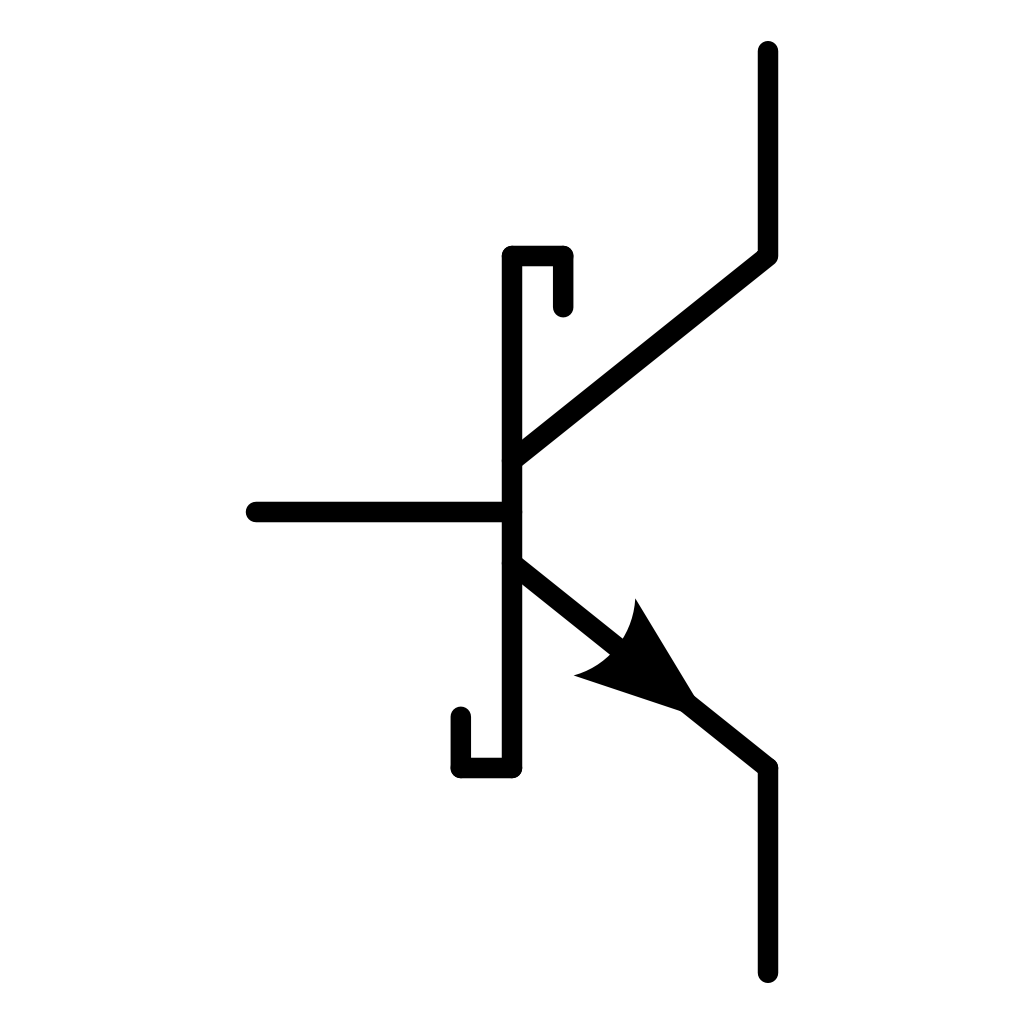
\includegraphics[width=0.1\textwidth]{../EJ2/Recursos/schottky_transistor_symbol} &
        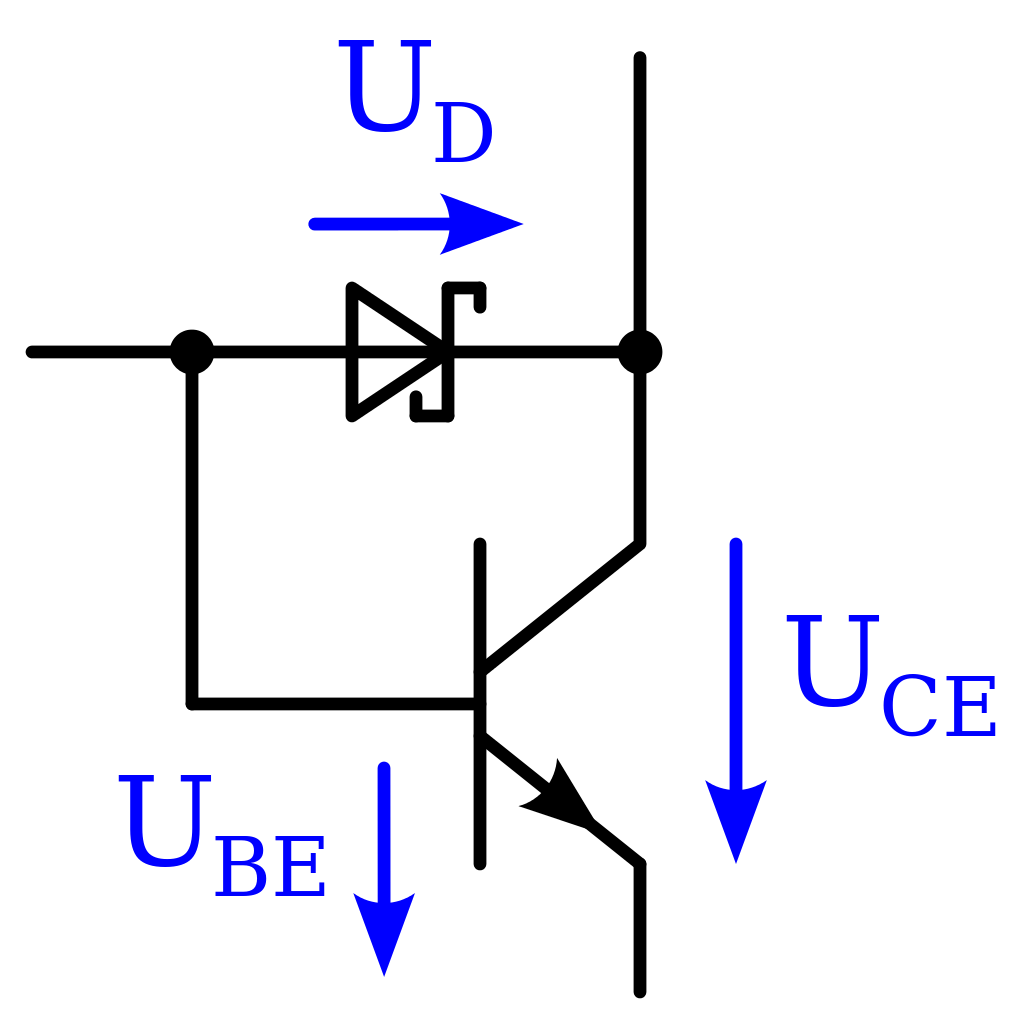
\includegraphics[width=0.1\textwidth]{../EJ2/Recursos/schottky_transistor_circuit}
    \end{tabular}
    \caption{Símbolo y circuito de transistor Schottky.}
    \label{fig:schottky_transistor_symbol_and_circuit_ex5}
\end{figure}

Tal y como fue mencionado en el inicio de esta sección, en este trabajo se estudiará la compatibilidad entre las tecnologías a través de sus márgenes de ruido.
Esto significa que, en términos de interconexión, una compuerta solo será compatible con otra de otra tecnología, si el rango de valores de salida de la primera está 
incluido en el rango de entrada de la segunda. \\
En las figuras \ref{fig:compatible_v_non_compatible_ex5} y \ref{fig:compatible_v_non_compatible_2_ex5} pueden apreciarse los casos que pueden presentarse que significarán la compatibilidad o no entre las compuertas.
De ellos se extrae que las compuertas serán compatibles solo en el caso en que $V_{OH} \leq V_{IH}$ y $V_{OL} \geq V_{IL}$.

\begin{figure}[H]
    \centering
    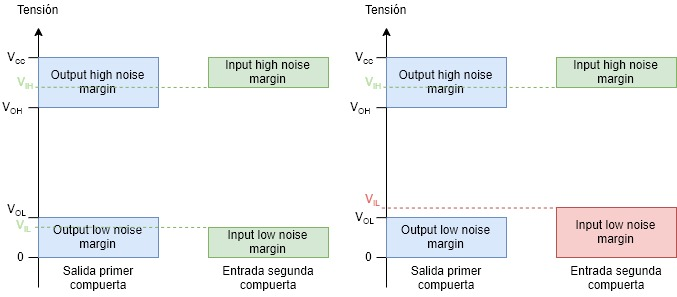
\includegraphics[width=0.8\textwidth]{../EJ2/Recursos/compatible_gates}
    \caption{Compatibilidad de compuertas.}
    \label{fig:compatible_v_non_compatible_ex5}
\end{figure}

\begin{figure}[H]
    \centering
    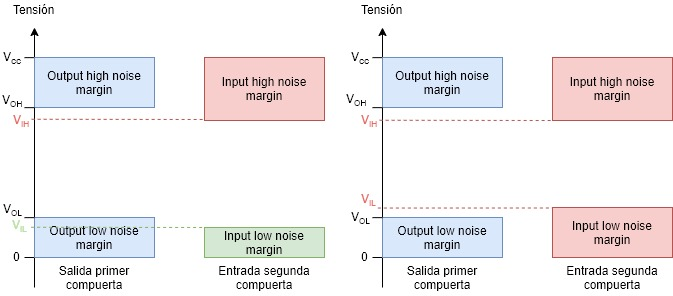
\includegraphics[width=0.8\textwidth]{../EJ2/Recursos/incompatible_gates}
    \caption{Compatibilidad de compuertas.}
    \label{fig:compatible_v_non_compatible_2_ex5}
\end{figure}

Con respecto al fanout, el mismo refiere